\section{Modelagem}
Segundo \citeonline{SOMMERVILLE:2019}, a modelagem de sistemas é definida como ``um processo de desenvolvimento de modelos abstratos de um sistema, cada um apresentando uma visão diferente do mesmo''. Para isso, descreve também que são geralmente usadas notações gráficas baseadas nos tipos de diagrama em \acs{uml} durante o processo de engenharia de requisitos ``para ajudar a derivar os requisitos detalhados de um sistema; durante o processo [...]; e depois da implementação, para documentar a estrutura e operação do sistema'' \cite{SOMMERVILLE:2019}. 

\subsection{Diagrama de Casos de Uso}
De acordo com \citeonline{umlGuedes}, o diagrama de casos de uso \acs{uml} é descrito como:

\begin{citacao}
O diagrama de casos de uso [...] tem por objetivo apresentar uma visão externa geral das funcionalidades que o sistema deverá oferecer aos usuários, sem se preocupar com a questão de como tais funcionalidades serão implementadas. [...] É de grande auxílio para a identificação e compreensão dos requisitos do sistema, ajudando a especificar, visualizar e documentar as características, funções e serviços do sistema desejados pelo usuário \cite{umlGuedes}.
\end{citacao}

Logo, a \autoref{diagrama_CasosUso} representa os casos de uso do projeto de sistema \gls{ifriends}.

\begin{figure}[htb]
\centering
\caption{Diagrama de Casos de Uso}
\label{diagrama_CasosUso}
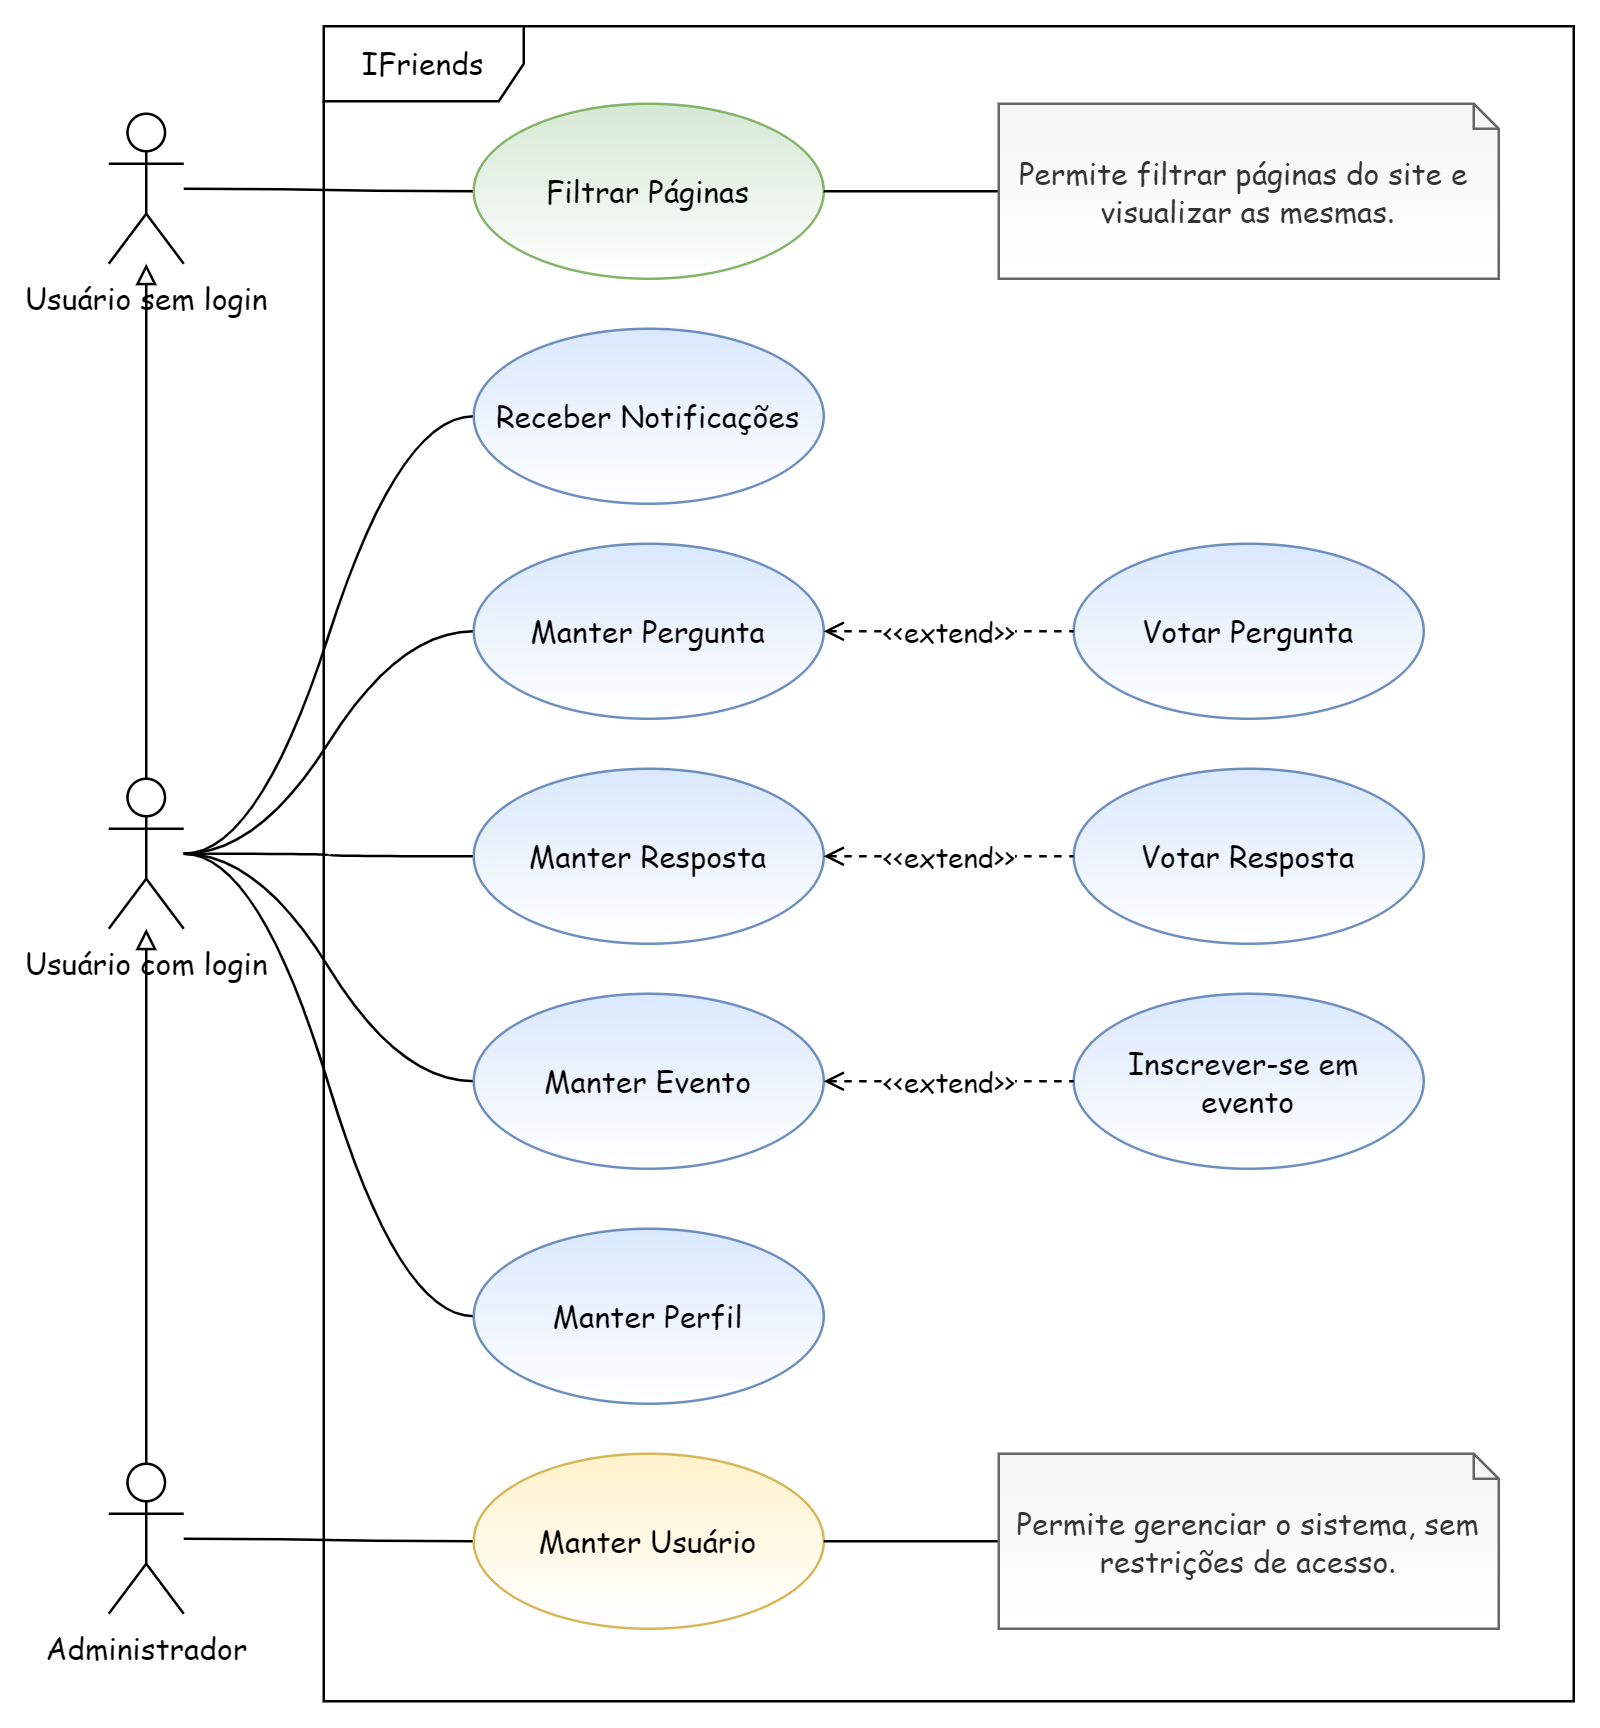
\includegraphics[width=1.0\textwidth]{anexos/Imagens_Diagramas/CasosDeUso_IFriends.png}
\fonte{Os autores.}
\end{figure}
\FloatBarrier


%\subsection{Diagrama de Classes}
% É necessário?

\subsection{Diagrama de Entidade e Relacionamento}

De acordo com \citeonline{leal2015linguagem}, a abordagem entidade-relacionamento é a técnica de modelagem de dados mais difundida e utilizada e representa a modelo conceitual do banco de dados. Nela, a estrutura do banco de dados é descrita como coleção de entidades, relacionamentos e representada graficamente por meio do Diagrama Entidade Relacionamento.

Através dele, é possível descrever um subconjunto do mundo real que será retratado no banco de dados com um alto nível de abstração. Além disso, o modelo Entidade Relacionamento é um modelo formal e caracteriza-se por ter uma grande capacidade semântica, o que garante que todos possam ter o mesmo entendimento \cite{leal2015linguagem}.

A \autoref{diagrama_EntidadeRelacionamento} representa o \ac{der} do projeto de sistema \gls{ifriends}.

\begin{figure}[htb]
\centering
\caption{Diagrama de Entidade e Relacionamento}
\label{diagrama_EntidadeRelacionamento}
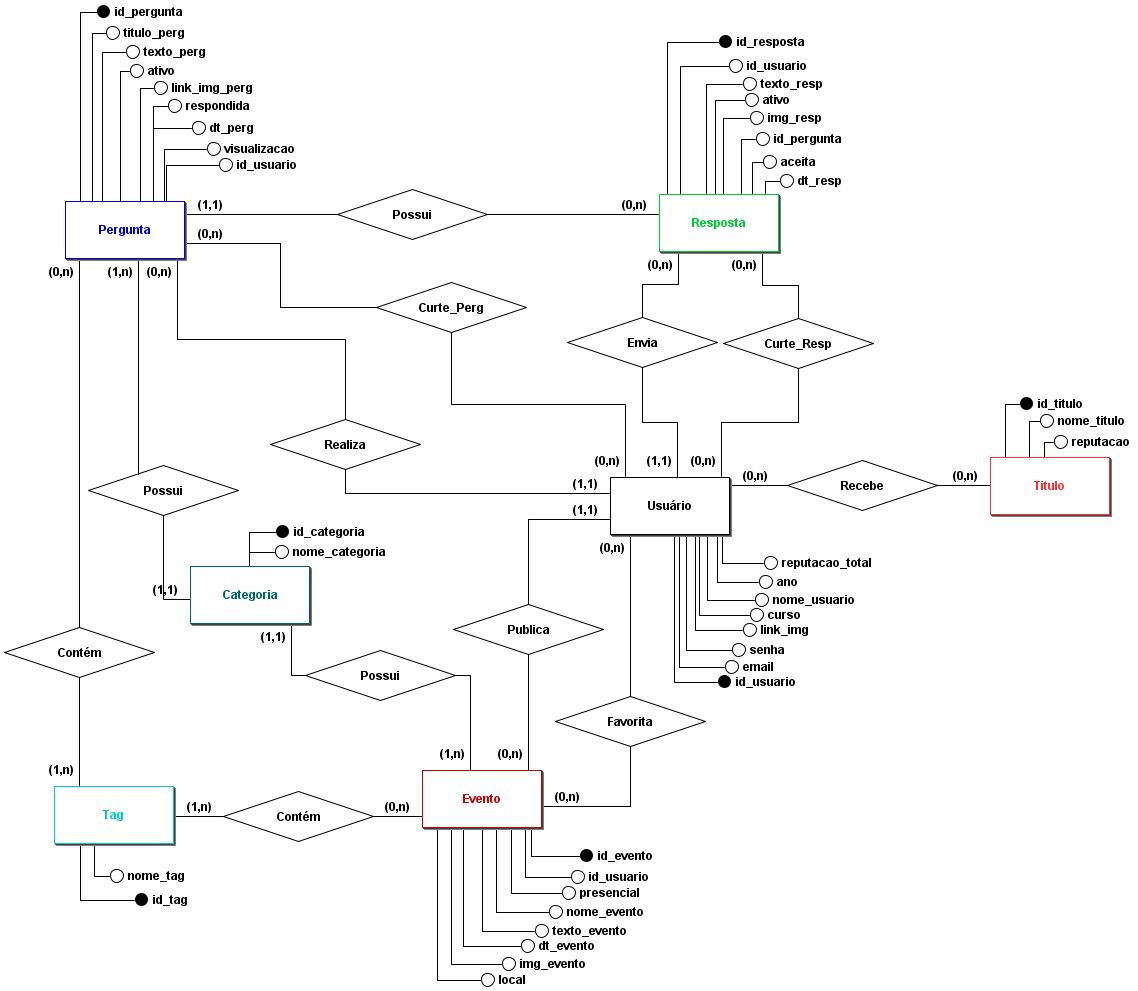
\includegraphics[width=1.0\textwidth]{anexos/Imagens_Diagramas/DER_IFriends.png}
\fonte{Os autores.}
\end{figure}
\FloatBarrier


\subsection{Diagrama de Tabelas Relacionais}

O Diagrama de Tabelas Relacionais \acs{dtr} representa o modelo lógico do Banco de Dados. Segundo \citeonline{utilidadepublica:201?}, através do modelo lógico é representado de maneira mais clara as entidades e os relacionamentos, pois considera algumas limitações e implementa recursos como adequação de padrão e nomenclatura, define as chaves primárias e estrangeiras, normalização, integridade referencial, entre outras.

Deste modo, a \autoref{diagrama_TabelasRelacionais} representa o \ac{dtr} do projeto de sistema \gls{ifriends}.

\begin{figure}[htb]
\centering
\caption{Diagrama de Tabelas Relacionais}
\label{diagrama_TabelasRelacionais}
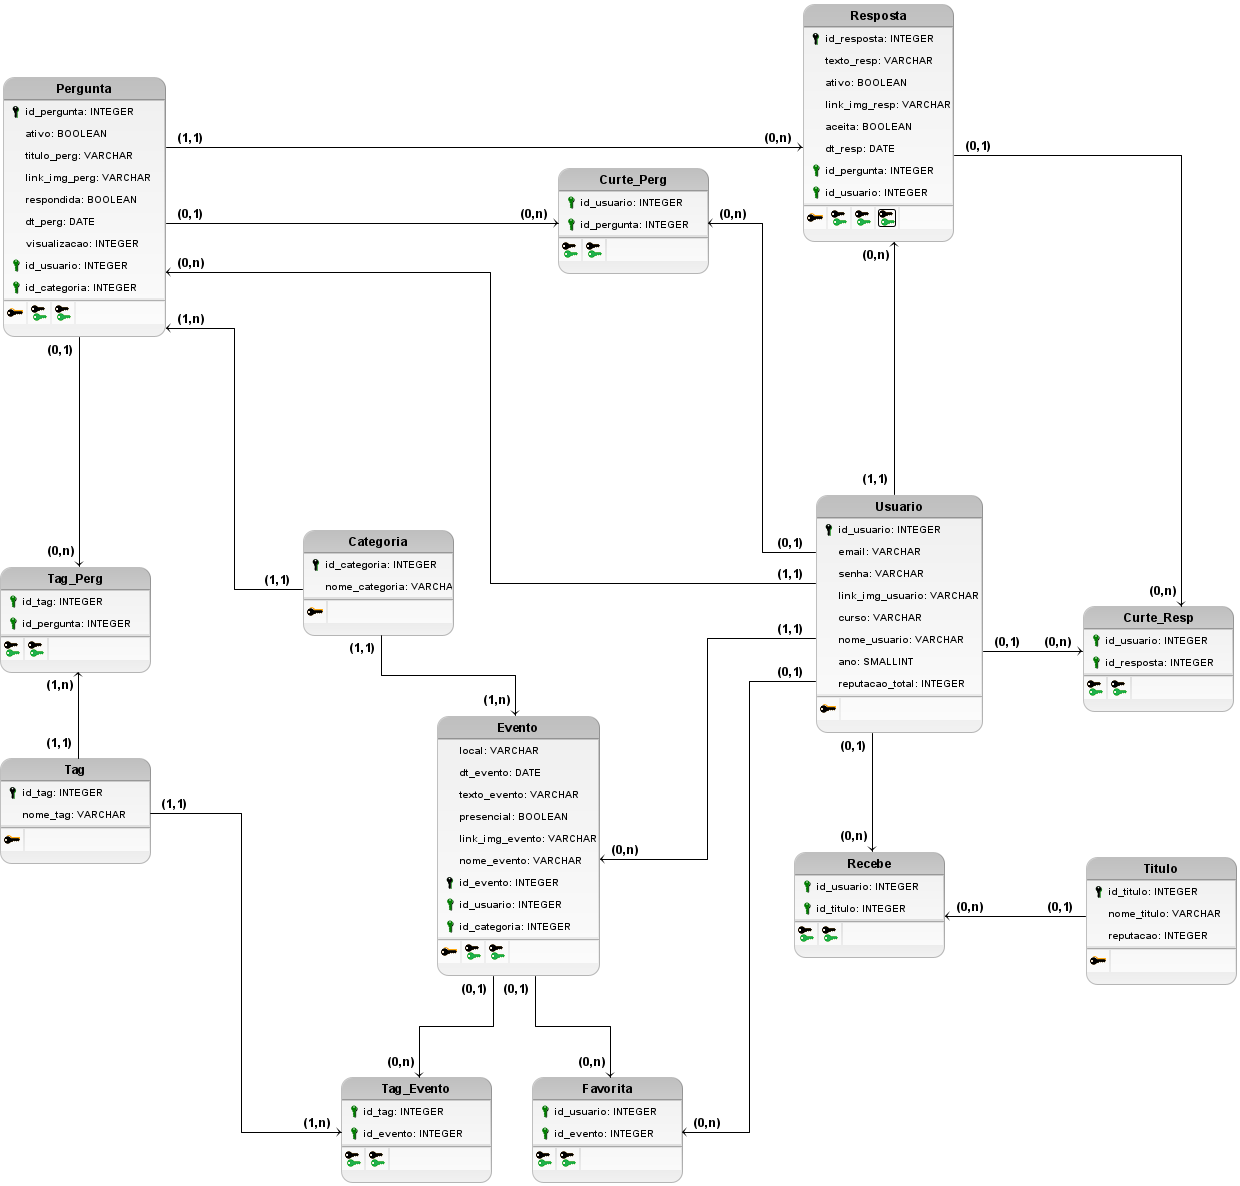
\includegraphics[width=0.9\textwidth]{anexos/Imagens_Diagramas/DTR_IFriends.png}
\fonte{Os autores.}
\end{figure}
\FloatBarrier

\subsection{Dicionário de Dados}

O Dicionário de dados é responsável por armazenar as informações de configuração do banco de dados e as estruturas que compõem suas respectivas tabelas. As estruturas definem os campos e suas propriedades \cite{alvesbanco}.

Conforme \citeonline{date2004introdução}, o Dicionário de dados é o lugar em que – dentre outras coisas – todos os diversos esquemas (externo, conceitual, interno) e todos os mapeamentos correspondentes são mantidos.

O Dicionário de dados contém os metadados, dados que explicam dados, com relação aos diversos objetos que são de interesse do próprio sistema. Exemplos desses objetos incluem índices, usuários, restrições de integridade, restrições de segurança, e assim por diante, informações que essenciais para que o sistema faça seu trabalho apropriadamente \cite{date2004introdução}.

De tal modo, abaixo encontram-se os quadros que representam o \ac{dd} das tabelas de banco de dados do projeto \gls{ifriends}.

%%%%%%%%% Tabela usuario
\def\arraystretch{1.5}

\begin{quadro}[htb]
\centering
\ABNTEXfontereduzida
\caption[Usuário]{Usuário.}
\begin{tabular}{|>{\Centering}m{3cm}|>{\Centering}m{1.75cm}|>{\Centering}m{1.6cm}|>{\Centering}m{1.15cm}|>{\Centering}m{1.25cm}|m{4.5cm}|}
\hline
\thead{Atributo} & \thead{Tipo} & \thead{Tamanho} & \thead{Nulo} & \thead{Chave} & \thead{Descrição}\\
\hline

id\_usuario & INT & 11 & N & PK & Chave primária do usuário \\ \hline
email & VARCHAR & 50 & N &  & E-mail institucional do usuário \\ \hline
senha & VARCHAR & 50 & N &  & Senha de acesso ao sistema \\ \hline
link\_img & TEXT &  & S &  & link da imagem de perfil \\ \hline
curso & VARCHAR & 50 & S &  & Curso atual \\ \hline
nome\_usuario & VARCHAR & 120 & N &  & Nome do usuário \\ \hline
ano & INT & 1 & S &  & Ano que o usuário cursa, ex.: 1\textdegree ano \\ \hline
reputacao\_total & INT & 11 & N  &  & Pontuação da reputação do usuário \\ \hline

\end{tabular}\legend{Fonte: Os autores}
\end{quadro}
\FloatBarrier 

%%%%%%%% Tabela usuario - pergunta
\def\arraystretch{1.5}

\begin{quadro}[htb]
\centering
\ABNTEXfontereduzida
\caption[Usuário\_Pergunta]{Usuário\_Pergunta.}
\label{quadro-dicionario-dados}
\begin{tabular}{|>{\Centering}m{3cm}|>{\Centering}m{1.75cm}|>{\Centering}m{1.6cm}|>{\Centering}m{1.15cm}|>{\Centering}m{1.25cm}|m{4.5cm}|}
\hline
\thead{Atributo} & \thead{Tipo} & \thead{Tamanho} & \thead{Nulo} & \thead{Chave} & \thead{Descrição}\\
\hline

id\_usuario & INT & 11 & N & FK & Chave estrangeira no usuário \\ \hline
id\_pergunta & INT & 11 & N & FK & Chave estrangeira na pergunta \\ \hline

\end{tabular}\legend{Fonte: Os autores}
\end{quadro}
\FloatBarrier 

%\clearpage

%usuario - resposta
\def\arraystretch{1.5}

\begin{quadro}[htb]
\centering
\ABNTEXfontereduzida
\caption[Usuário\_Resposta]{Usuário\_Resposta.}
\label{quadro-dicionario-dados}
\begin{tabular}{|>{\Centering}m{3cm}|>{\Centering}m{1.75cm}|>{\Centering}m{1.6cm}|>{\Centering}m{1.15cm}|>{\Centering}m{1.25cm}|m{4.5cm}|}
\hline
\thead{Atributo} & \thead{Tipo} & \thead{Tamanho} & \thead{Nulo} & \thead{Chave} & \thead{Descrição}\\
\hline

id\_usuario & INT & 11 & N & FK & Chave estrangeira no usuário \\ \hline
id\_resposta & INT & 11 & N & FK & Chave estrangeira na resposta \\ \hline

\end{tabular}\legend{Fonte: Os autores}
\end{quadro}
\FloatBarrier 

%usuario - Titulo
\def\arraystretch{1.5}

\begin{quadro}[htb]
\centering
\ABNTEXfontereduzida
\caption[Usuário\_Título]{Usuário\_Título.}
\label{quadro-dicionario-dados}
\begin{tabular}{|>{\Centering}m{3cm}|>{\Centering}m{1.75cm}|>{\Centering}m{1.6cm}|>{\Centering}m{1.15cm}|>{\Centering}m{1.25cm}|m{4.5cm}|}
\hline
\thead{Atributo} & \thead{Tipo} & \thead{Tamanho} & \thead{Nulo} & \thead{Chave} & \thead{Descrição}\\
\hline

id\_usuario & INT & 11 & N & FK & Chave estrangeira no usuário \\ \hline
id\_titulo & INT & 11 & N & FK & Chave estrangeira no titulo \\ \hline

\end{tabular}\legend{Fonte: Os autores}
\end{quadro}
\FloatBarrier 


%Titulo
\def\arraystretch{1.5}

\begin{quadro}[htb]
\centering
\ABNTEXfontereduzida
\caption[Título]{Título.}
\label{quadro-dicionario-dados}
\begin{tabular}{|>{\Centering}m{3cm}|>{\Centering}m{1.75cm}|>{\Centering}m{1.6cm}|>{\Centering}m{1.15cm}|>{\Centering}m{1.25cm}|m{4.5cm}|}
\hline
\thead{Atributo} & \thead{Tipo} & \thead{Tamanho} & \thead{Nulo} & \thead{Chave} & \thead{Descrição}\\
\hline

id\_titulo & INT & 11 & N & PK & Chave primária do título \\ \hline
nome\_titulo & VARCHAR & 50 & N &  & Nome do título \\ \hline
reputacao & INT & 11 & N & & Acumulo da pontuação \\\hline

\end{tabular}\legend{Fonte: Os autores}
\end{quadro}
\FloatBarrier 
%\clearpage

%Resposta
\def\arraystretch{1.5}

\begin{quadro}[htb]
\centering
\ABNTEXfontereduzida
\caption[Resposta]{Resposta.}
\label{quadro-dicionario-dados}
\begin{tabular}{|>{\Centering}m{3cm}|>{\Centering}m{1.75cm}|>{\Centering}m{1.6cm}|>{\Centering}m{1.15cm}|>{\Centering}m{1.25cm}|m{4.5cm}|}
\hline
\thead{Atributo} & \thead{Tipo} & \thead{Tamanho} & \thead{Nulo} & \thead{Chave} & \thead{Descrição}\\ \hline

id\_resposta & INT & 11 & N & PK & Chave primária da resposta \\ \hline
id\_usuario & INT & 11 & N & FK  & Chave estrangeira de usuário \\ \hline
id\_pergunta & INT & 11 & N & FK & Chave estrangeira de pergunta \\ \hline
texto\_resp & TEXT &  & N &  & Conteúdo da resposta \\ \hline
ativo & BOOLEAN & & N & & Resposta ativa ou não \\ \hline
img\_resp & TEXT & & S & & Imagem da resposta \\ \hline
aceita & BOOLEAN & & N & & Se a resposta foi aceita como solução válida para o autor da pergunta \\ \hline
dt\_resposta & DATE & 50 & N & & Data em que a resposta foi publicada \\ \hline

\end{tabular}\legend{Fonte: Os autores}
\end{quadro}
\FloatBarrier 

%Tag
\def\arraystretch{1.5}

\begin{quadro}[htb]
\centering
\ABNTEXfontereduzida
\caption[Tag]{Tag.}
\label{quadro-dicionario-dados}
\begin{tabular}{|>{\Centering}m{3cm}|>{\Centering}m{1.75cm}|>{\Centering}m{1.6cm}|>{\Centering}m{1.15cm}|>{\Centering}m{1.25cm}|m{4.5cm}|}
\hline
\thead{Atributo} & \thead{Tipo} & \thead{Tamanho} & \thead{Nulo} & \thead{Chave} & \thead{Descrição}\\
\hline

id\_tag & INT & 3 & N & PK & Chave primária da tag \\ \hline
nome\_tag & VARCHAR & 50 & N &  & Nome da tag \\ \hline

\end{tabular}\legend{Fonte: Os autores}
\end{quadro}
\FloatBarrier 
%\clearpage

%Pergunta
\def\arraystretch{1.5}

\begin{quadro}[htb]
\centering
\ABNTEXfontereduzida
\caption[Pergunta]{Pergunta.}
\label{quadro-dicionario-dados}
\begin{tabular}{|>{\Centering}m{3cm}|>{\Centering}m{1.75cm}|>{\Centering}m{1.6cm}|>{\Centering}m{1.15cm}|>{\Centering}m{1.25cm}|m{4.5cm}|}
\hline
\thead{Atributo} & \thead{Tipo} & \thead{Tamanho} & \thead{Nulo} & \thead{Chave} & \thead{Descrição}\\ \hline

id\_pergunta & INT & 11 & N & PK & Chave primária da pergunta \\ \hline
id\_usuario & INT & 11 & N & FK  & Chave estrangeira de usuário \\ \hline
dt\_perg & DATE &  & N & & Data da pergunta \\ \hline
titulo\_perg & VARCHAR & 50 & N & & Título da pergunta \\ \hline
texto\_perg & TEXT & & N & & Descrição da pergunta \\ \hline
ativo & BOOLEAN & & N & & Pergunta ativa ou não \\ \hline
link\_img\_perg & TEXT & & S & & Link da imagem da pergunta \\ \hline
respondida & BOOLEAN & & N & & Se a pergunta já teve uma resposta útil a quem perguntou \\ \hline
visualizações & INT & 5 & N & & Quantidade de visualizações da pergunta \\ \hline

\end{tabular}\legend{Fonte: Os autores}
\end{quadro}
\FloatBarrier 


%Tag - Pergunta
\def\arraystretch{1.5}

\begin{quadro}[htb]
\centering
\ABNTEXfontereduzida
\caption[Tag\_Pergunta]{Tag\_Pergunta.}
\label{quadro-dicionario-dados}
\begin{tabular}{|>{\Centering}m{3cm}|>{\Centering}m{1.75cm}|>{\Centering}m{1.6cm}|>{\Centering}m{1.15cm}|>{\Centering}m{1.25cm}|m{4.5cm}|}
\hline
\thead{Atributo} & \thead{Tipo} & \thead{Tamanho} & \thead{Nulo} & \thead{Chave} & \thead{Descrição}\\ \hline

id\_assunto & INT & 11 & N & FK & Chave estrangeira no assunto \\ \hline
id\_pergunta & INT & 11 & N & FK & Chave estrangeira na pergunta \\ \hline

\end{tabular}\legend{Fonte: Os autores}
\end{quadro}
\FloatBarrier 
%\clearpage

%Tag - Evento
\def\arraystretch{1.5}

\begin{quadro}[htb]
\centering
\ABNTEXfontereduzida
\caption[Tag\_Evento]{Tag\_Evento.}
\label{quadro-dicionario-dados}
\begin{tabular}{|>{\Centering}m{3cm}|>{\Centering}m{1.75cm}|>{\Centering}m{1.6cm}|>{\Centering}m{1.15cm}|>{\Centering}m{1.25cm}|m{4.5cm}|}
\hline
\thead{Atributo} & \thead{Tipo} & \thead{Tamanho} & \thead{Nulo} & \thead{Chave} & \thead{Descrição}\\ \hline

id\_assunto & INT & 11 & N & FK & Chave estrangeira no assunto \\ \hline
id\_evento & INT & 11 & N & FK & Chave estrangeira no evento \\ \hline

\end{tabular}\legend{Fonte: Os autores}
\end{quadro}
\FloatBarrier 

%evento
\def\arraystretch{1.5}

\begin{quadro}[htb]
\centering
\ABNTEXfontereduzida
\caption[Evento]{Evento.}
\label{quadro-dicionario-dados}
\begin{tabular}{|>{\Centering}m{3cm}|>{\Centering}m{1.75cm}|>{\Centering}m{1.6cm}|>{\Centering}m{1.15cm}|>{\Centering}m{1.25cm}|m{4.5cm}|}
\hline
\thead{Atributo} & \thead{Tipo} & \thead{Tamanho} & \thead{Nulo} & \thead{Chave} & \thead{Descrição}\\
\hline

id\_evento & INT & 11 & N & PK & Chave primária do evento \\ \hline
id\_usuario & INT & 11 & S & FK  & Chave estrangeira de usuário \\ \hline
presencial & char & 1 & N & & Local do evento, sendo presencial, online ou ambos \\ \hline
nome\_evento & VARCHAR & 50 & N & & Nome do evento \\ \hline
texto\_evento & TEXT &  & N & & Descrição sobre o evento \\ \hline
dt\_evento & DATE & & N & & Data que o evento ocorrerá \\ \hline
img\_evento & TEXT &  & S & & Imagem do evento \\ \hline
local & TEXT & & N & & Local onde será realizado, tanto presencial como online \\ \hline
\end{tabular}\legend{Fonte: Os autores}
\end{quadro}
\FloatBarrier 

%Categoria
\def\arraystretch{1.5}

\begin{quadro}[htb]
\centering
\ABNTEXfontereduzida
\caption[Categoria]{Categoria.}
\label{quadro-dicionario-dados}
\begin{tabular}{|>{\Centering}m{3cm}|>{\Centering}m{1.75cm}|>{\Centering}m{1.6cm}|>{\Centering}m{1.15cm}|>{\Centering}m{1.25cm}|m{4.5cm}|}
\hline
\thead{Atributo} & \thead{Tipo} & \thead{Tamanho} & \thead{Nulo} & \thead{Chave} & \thead{Descrição}\\
\hline

id\_categoria & INT & 11 & N & PK & Chave primária da categoria \\ \hline
nome\_categoria & INT & 50 & N & FK & Nome da categoria \\ \hline

\end{tabular}\legend{Fonte: Os autores}
\end{quadro}
\FloatBarrier 

%\clearpage